%----------------------------------------------------------------
%
%  File    :  survey-intro.tex
%
%  Author  :  Keith Andrews, IICM, TU Graz, Austria
% 
%  Created :  27 May 1993
% 
%  Changed :  16 Nov 2010
% 
%----------------------------------------------------------------


\chapter{Screen Readers}

\label{chap:Intro}



Screen readers are software applications, primarily used by visually impaired people. Screen readers convert web content (text, buttons, images, and other elements) into speech or braille output. Screen readers attempt to convey what visually non-impaired people see on a display via non-visual means like text-to-speech, sound icons, or a braille device.

In May - June 2021, WebAIM surveyed preferences of screen reader users. They received 1568 valid responses. Figure \ref{fig:screen-readers-piechart} shows the primary screen readers preferences. The majority of users uses JAWS and NVDA screen readers as their primary screen reader. Figure \ref{fig:screen-readers-line} shows historical trends for primary screen reader usage. After a decade of decreases in primary usage, JAWS is once again the most used screen reader, with NVDA and VoiceOver both decreasing in primary usage over the last two years.

In this paper, we focus on JAWS, NVDA, VoiceOver, Narrator, and TalkBack screen readers.

\begin{figure}[tp]
\centering
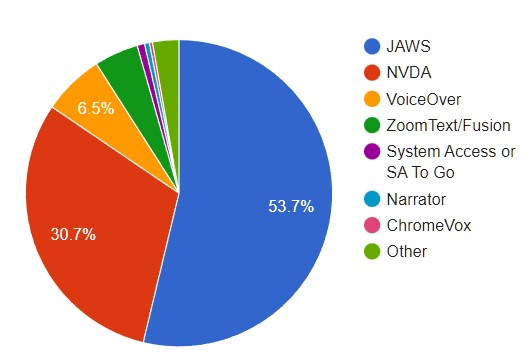
\includegraphics[keepaspectratio,width=\linewidth,height=\halfh]
{images/screen-readers-piechart.jpg}

\caption[Primary screen reader]{
Primary screen reader.
\imgcredit{Image extracted from WebAIM. ©2022 WebAIM.}
}
\label{fig:screen-readers-piechart}
\end{figure}

\begin{figure}[tp]
\centering
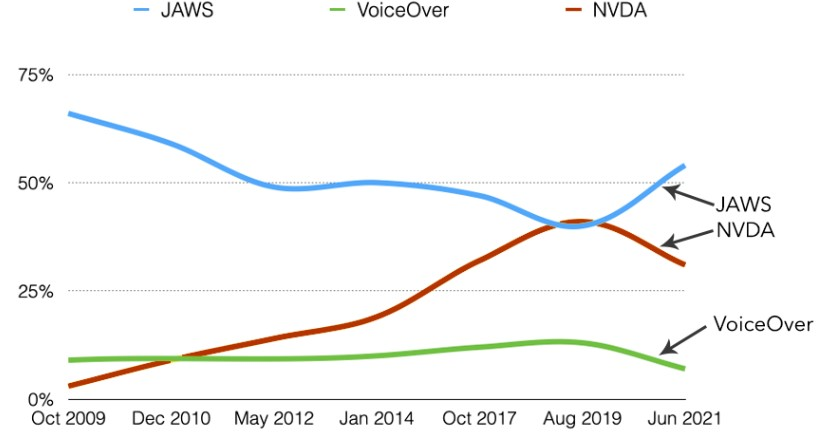
\includegraphics[keepaspectratio,width=\linewidth,height=\halfh]
{images/screen-readers-line.jpg}

\caption[Historical trends for primary screen reader]{
Historical trends for primary screen reader.
\imgcredit{Image extracted from WebAIM. ©2022 WebAIM.}
}
\label{fig:screen-readers-line}
\end{figure}




\section{JAWS}

Lorem ipsum dolor sit amet...

\section{NVDA}

Lorem ipsum dolor sit amet...

\section{VoiceOver}

Lorem ipsum dolor sit amet...

\section{Narrator}

Lorem ipsum dolor sit amet...

\section{TalkBack}

Lorem ipsum dolor sit amet...

\section{Screen Readers Comparison}

Lorem ipsum dolor sit amet...


